\problemname{Xorxorxor}

\begin{center}
  \begin{figure}[h!]
    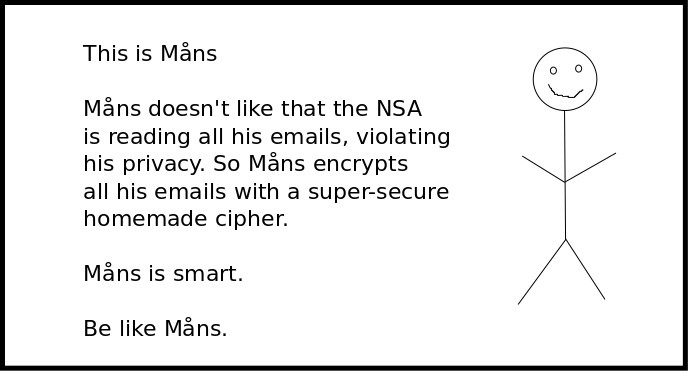
\includegraphics[width=\textwidth]{mans.png}
  \end{figure}
\end{center}

Måns has come up with a brilliant cipher to protect himself from villains trying to read his email. His cipher works as follows. First, he uses the ASCII character encoding to represent each character in his email as a number between 0--127. Then he chooses a key consisting of $K$ bytes in the range 0--255. If the key consists of bytes $a_0, a_1, a_2, ... a_{k - 1}$, and his email consists of bytes $b_0, b_1, b_2, ...$ then the encryption
consists of bytes $k_i = b_i \oplus a_{(i \mod K)}$, where $\oplus$ is a \href{https://en.wikipedia.org/wiki/Bitwise\_operation#XOR}{bitwise XOR} over the 8 bits of the byte, and $i \mod K$ is the \href{https://en.wikipedia.org/wiki/Modulo\_operation}{usual modulo operation}. Finally, he encodes each byte as two characters in base 16 (\href{https://en.wikipedia.org/wiki/Hexadecimal}{hexadecimal}).

Given Måns's encrypted message, determine what the original message looked like.

\section*{Input}
The input consists of a number of lines -- the encrypted message. Note that any line breaks are only present to make the input easier to read and should not be considered in the problem.

Each original message consists of at least 500 and at most 1050 characters.

\section*{Output}
You should output, character by character, Måns's original message.

\section*{Scoring}

\begin{enumerate}
	\item[6 points] $K = 1$, the message consists only of lowercase letters $a$--$z$ and spaces.
	\item[10 points] $K = 1$.
  \item[12 points] $K \le 5$, the text consists to 70\% of the word \texttt{fisk}.
	\item[19 points] $K \le 5$, the message consists only of lowercase letters $a$--$z$ and spaces.
  \item[24 points] $K \le 5$.
	\item[33 points] $K \le 10$, the message consists only of lowercase letters $a$--$z$ and spaces.
  \item[41 points] $K \le 10$.
	\item[15 points] $K = 15$, the word ``flaggstangsknoppspoleringsmedel'' appears in the text.
\end{enumerate}

In all cases, real text has been encrypted, in either English, Swedish, or German. Any \href{https://en.wikipedia.org/wiki/Diacritics}{diacritical marks} have been removed.
